
\chapter{Security of third-party apps}

\section{App runtime}

The applications are intended to be run on a wide range of devices, with different hardware configurations.
The execution environment needs to be able to enforce access control and isolation.
To make it scalable, it is necessary to have an abstraction layer that would allow the apps to be run on different hardware configurations.
Moreover, the devices are very limited in resources, which makes it difficult to adapt the existing solutions such as Java virtual machine.
For those reasons, Garmin decided to create a custom virtual machine and a programming language.

However, creating a correct abstraction layer is a complex task.
It creates a large attack surface, and it is challenging to ensure that the implementation is correct.

\section{Preliminary analysis}
The existing research analysed the bytecode of the firmware running on the watch.
Unfortunately, the firmware is no longer available for download.
There is a chance that it would be possible to reverse engineer the watch hardware and extract the firmware from the device.
However, it would require an extensive amount of time and resources.
Another option would be to investigate the protocol used to download a new firmware version.
It would require additional time and there is no guarantee that it would be possible to download the full firmware.
Performing a static analysis of the firmware would be a very time-consuming and tedious process.
It would require decompiling and analysing the code of the virtual machine, without any documentation, any meaningful names of the variables and functions.

In the end, I decided to perform the analysis on the simulator provided by Garmin.
As it runs directly on the computer, it is possible to use different approaches such as dynamic analysis.
This leaves more flexibility and allows for a more in-depth analysis of the software.
The simulator is supposed to guarantee proper isolation, so escaping the sandbox could be a potential vulnerability being a threat to the host machine.
Additionally, there is a chance that parts of the code are reused in the firmware running on the watch and the findings would be applicable to the real device.

\section{Permissions}
\begin{figure}[h]
    \centering
    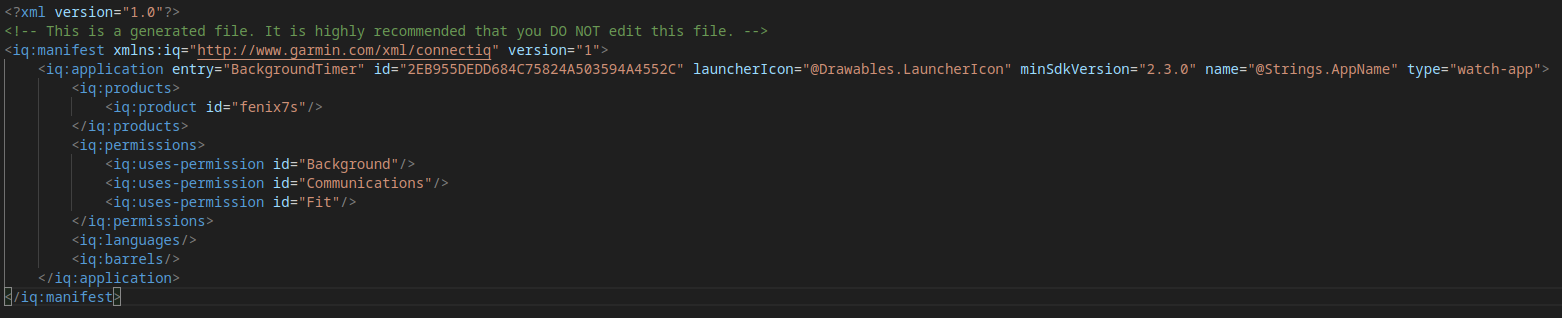
\includegraphics[width=1\linewidth]{../../images/garmin-app-manifest}
    \caption{Garmin third-party app manifest}
    \label{fig:garmin-app-manifest}
\end{figure}
Third-party apps can interact with the watch by using the API provided by the SDK\@.
The API is divided into several modules, each of them providing different functionality.

Garmin differentiates five different types of apps, e.g.\ watch app, watch face.
The type determines which modules are available for the app.
Some functionalities can be considered sensitive, such as GPS location, heart rate, or access to the internet.
Because of that, Garmin implemented a permission system, where different permissions grant access to different modules.
The app has to define in the manifest file which permissions it requires, and the user has to accept them before installing the app.
The manifest file is presented in the figure~\ref{fig:garmin-app-manifest}.

The system offers some granularity, and can give the user a general overview of what the app can do.
However, a few, potentially sensitive modules don't require any permissions.
For example, the app can access several basic activity metrics such as heart rate, steps, calories without any permissions.
Moreover, in February 2023, Garmin introduced a new module: Complications.
It is a publish/subscribe model that allows for the apps to publish different metrics, so that they would be accessible for any watch face.
While it makes the access to different metrics more flexible and accessible, it also removes the granularity of the permissions.
Every app can potentially publish very sensitive data, without the user being aware of it.
Then every watch face can access all this data if it requests \textit{Complications} permission.

Watch faces often require several permissions to be able to display different metrics.
As watch faces are usually downloaded based on the personal design preferences, users are likely to install some that are not very popular.
This makes it difficult to build a trust relationship with the developer.
Which means that the only protection for the user is the permission system and Garmin review process.

A potential improvement would be to create an API for watch faces that would not require any permissions.
The watch face could describe the design, and the watch could be responsible for displaying the metrics.

\section{Building process}
In order to understand the runtime environment, I started with the analysis of the building process.
As it was mentioned, it is recommended to use Visual Studio Code with the extension provided by Garmin.
The program is written in Monkey C language.
For testing purposes, the app can be run on a simulator or a real device.
The extension provides a user interface to automatically install the app on the simulator.
It is also possible to generate a binary PRG file that can be installed on the watch.
Before the app can be installed on the watch, it has to be signed by the developer.

During the compilation, the code is translated to mid-level intermediate representation (MIR).
The files containing the representations could be used for better understanding of the final artefact.

Visual Studio calls the compiler, which is a jar file called \textit{monkeybrains.jar}.
The compiler is written in Java, which makes the analysis of the code relatively straightforward.
Nonetheless, it is a complicated process consisting of several stages.
For the analysis, I decided to use the JADX decompiler\footnote{\url{https://github.com/skylot/jadx}}.

After loading the jar file, I noticed that a large part of the relevant code is not obfuscated.
Then I proceeded to analyse the code.
The following classes are of particular interest:
\begin{itemize}
    \item \texttt{com.garmin.monkeybrains.compiler2.Compiler2} — main class responsible for the compilation process.
    \item \texttt{com.garmin.connectiq.common.monkeyc.AssemblerOpcode} — contains a list of instructions in the final bytecode.
    \item \texttt{com.garmin.connectiq.common.signing.SigningUtils} — class responsible for signing the app, described in more detail in the section~\ref{subsec:signing}.
\end{itemize}
Additionally, the SDK provides a mapping of all API methods to the number values.
This is probably used by the virtual machine to identify the method that should be called.

I was able to find the code responsible for signing the application.
It is described in more detail in the section~\ref{subsec:signing}.

\section{Signing} \label{subsec:signing}
Garmin requires that the apps are signed to be installed on the watch\cite{garmin-signing}.
The app has to be signed by the developer with their private key.
In order for the app to be updated, it has to be signed with the same key.
When the store has approved the app, it is additionally signed with the store signature.

The described process enforces that the app can be updated only by the developer having access to the original private key.
Additionally, when the app is downloaded from the store, the watch can verify that it has been approved by the store.

Based on the analysis of the compiler, class \texttt{SigningUtils} is responsible for signing the app.
It uses \texttt{java.security.Signature} class to generate the signature.
The signing algorithm uses SHA1 hash of the bytecode that is signed with a private RSA key.
The key is 4096 long, which is more than recommended.
For the signing, conventions described in PKCS \#1 v2.2 are used\cite{java-signature,pkcs}.
The pseudocode of the signing algorithm is presented in the listing~\ref{lst:signing}.
The signature computed by the store is generated in a similar way, does not include the modulus and exponent, and uses a different magic number.
The store probably uses the public key in the developer signature to verify and save it after the first upload of the app.
\begin{lstlisting}[caption={Pseudocode of the signing algorithm, developer signature},captionpos=b,label={lst:signing},language=Python]
    def sign_with_developer_signature():
        app_bytes = read_prg_file()
        app_bytes, terminator = remove_terminator(app_bytes)
        signature, modulus, exponent = compute_signature(app_bytes)

        dev_signature = byte_array()
        dev_signature.append(magic_number)
        dev_signature.append(signature_length)
        dev_signature.append(signature)
        dev_signature.append(modulus)
        dev_signature.append(exponent)

        signed_app = byte_array()
        signed_app.append_all(app_bytes, dev_signature, terminator)
        write_prg_file(signed_app)
\end{lstlisting}

SHA-1 is no longer considered secure against well-funded opponents.
NIST formally deprecated use of this hash function in 2011.
In 2020 there was a paper published demonstrating a chosen-prefix collision attack.
A potential vector of attack would be to create a malicious app with the same hash as the original app.
At the current state of the art, there is no viable solution to find a collision to a given hash for a chosen prefix.
However, the function has been already broken and in the upcoming years new attacks might be discovered.

\section{Modifying the executable}
\label{sec:modifying-the-executable}
To perform dynamic analysis of the virtual machine, it is useful to be able to edit the executable.
However, after changing the bytecode, it is necessary to sign the executable again.
With the knowledge gained from the previous section, I created a Kotlin script that signs the app again.

The code follows the same instructions as the original method in listing~\ref{lst:signing}.
The only difference is that the old signature is replaced with the new one.

\begin{figure}[h]
    \centering
    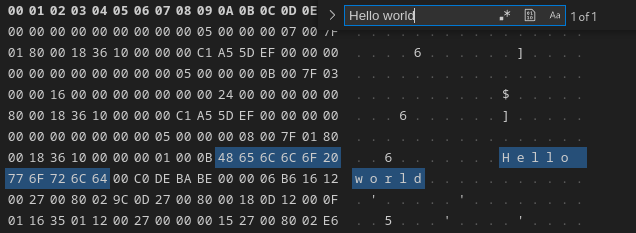
\includegraphics[width=0.7\linewidth]{../../images/app-hex-editor-hello-world}
    \caption{Prg file in hex editor}
    \label{fig:hello-world}
\end{figure}

To verify that the script works correctly, I created a simple app that shows a message 'Hello world'.
Then I opened the PRG file in a hex editor and searched for the message, as presented in the figure~\ref{fig:hello-world}.
Consequently, I modified the string and signed the app with the created script.
After installing the app on the watch and the simulator, the new message was displayed.
When trying to install the app without the new signature, the watch and the simulator would display an error message.

\section{Simulator}
Garmin SDK provides a simulator for testing the apps.
It is used by the Visual Studio Code extension to run the apps.
I found the executable in the SDK bin folder.
The file starts with ELF header, which means that it is a binary executable file.
To analyse bytecode, I decided to use Ghidra\footnote{\url{https://ghidra-sre.org/}}.
It is free and open-source software for reverse engineering.

After loading the file, a list of assembly instructions is displayed.
Fortunately, Ghidra has an option to analyse and decompile the code to C\@.

\begin{figure}[h]
    \centering
    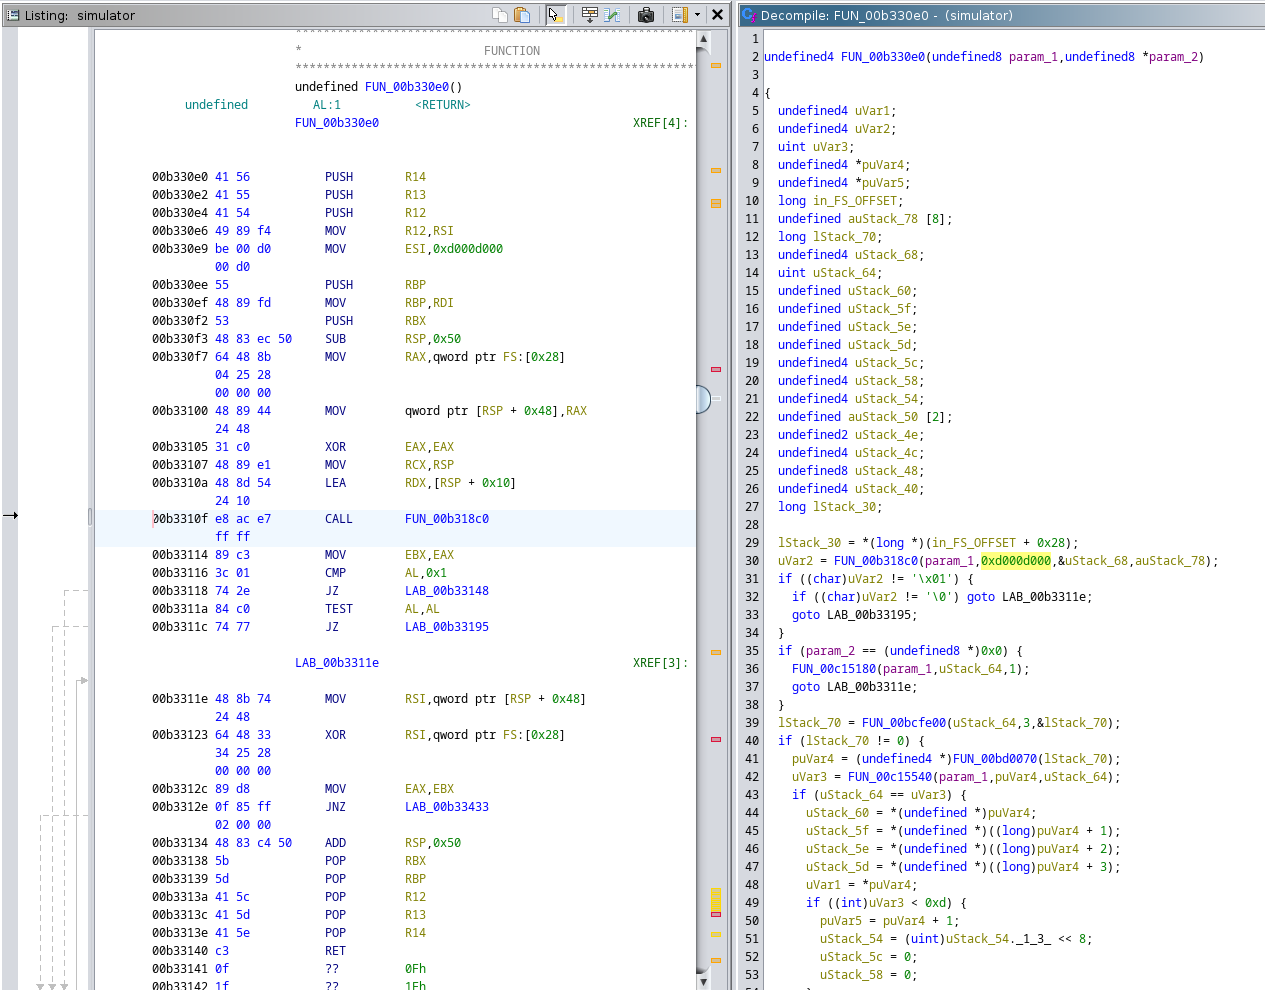
\includegraphics[width=0.7\linewidth]{../../images/ghidra}
    \caption{Simulator decompilation}
    \label{fig:concept}
\end{figure}

The header of the third-party apps is tagged with value `0xD000D000`\cite{broken-vm}.
Searching for it in the simulator binary reveals two references.

From this point, it would be theoretically possible to analyse the code and reverse engineer the virtual machine.
However, doing it without any documentation, where the names of the functions and variables are not known would be very challenging.
As it is not possible to do it in a reasonable amount of time, I decided to focus on fuzzing the virtual machine.
This is described in the section~\ref{sec:fuzzing}.

\section{Communication between the watch and the phone} \label{subsec:communication-watch-phone}

Garmin has multiple apps for managing the watch and the data.
As such, it is interesting to analyse the communication between them and the watch.
I analyzed the Manifest files in Connect IQ Store and Garmin Connect apps.
Both of them use Bluetooth permissions to connect with the watch.
Additionally, they define Garmin custom permissions as can be seen in the figure~\ref{fig:connect-iq-declared-permissions}.
The permissions have set protection level to `signature`(0x2), which means that only apps signed with the same key can use them.
They are used to be able to receive specific broadcasts, probably to communicate with themselves.
It is a functionality provided by Android and should offer an appropriate level of security.

\begin{figure}[h]
    \centering
    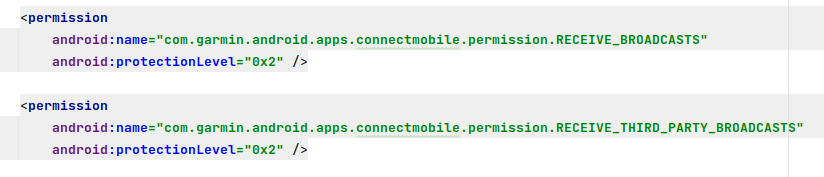
\includegraphics[width=1\linewidth]{../../images/android-declared-permissions}
    \caption{Declared permissions by Connect IQ Store}
    \label{fig:connect-iq-declared-permissions}
\end{figure}

When it comes to third-party apps, they can communicate with the phone by using the API provided by the SDK\@.
Garmin created SDK for Android and iOS that allows to create a companion mobile app for the watch app.
They created an example of watch and Android app that communicate with each other\footnote{\url{https://github.com/garmin/connectiq-android-sdk}}.
The Android SDK uses Broadcasts under the hood to communicate with Garmin Connect app.
The SDK allows the programmer to query for available Garmin devices connected to the phone.
Then it is possible to establish communication with a chosen app on the watch.

The first thing that can be noticed is that the SDK is able to get a list of all Garmin devices connected to the phone without any permissions.
They use Broadcasts that are available to all apps.
This creates a potential privacy issue, as any app can get the information if the user has a Garmin device connected to the phone.
Moreover, it is possible to get the information about the device, such as the model name.

Another issue is that the communication between the app on the watch and the companion app is not protected or encrypted.
The SDK offers a function to register a listener for events from the watch app, given the app ID\@.
However, when looking at the implementation, it is a wrapper around the Broadcasts.
It is possible to register a listener for all events from all apps.
This means that any app on the phone can listen to the messages from any watch app.
I did not find any mention in the documentation, that would warn the developers about this fact.

Following this finding, I decided to test this hypothesis.
I created a simple watch app that sends a message to the companion app.
Then, based on the SDK, I created an Android app that listens to all messages from all watch apps.
When I installed both apps, the Android app was able to receive the messages from the watch app with the information about the origin.

Having this information, I proceeded to investigate if it might be an issue for existing apps in the store.
Firstly, I looked into Spotify and Komoot apps.
Both of them are very popular and have a large number of downloads.
They have a full version of the app available on the phone and a companion app on the watch.
However, they do not use the mobile SDK provided by Garmin.
Instead, they connect to their servers directly.
It might be because it was easier to implement, or because they wanted to have more control over the communication.

Then I tried to find apps that use the mobile SDK provided by Garmin.
I found a developer 'r.485' that has published multiple apps in the store with the companion app on the phone.
However, when I installed the apps, they did not work correctly.

At this point, I decided to stop the investigation.
While it is a privacy issue, I could not find any apps that it would affect.


As Garmin already uses custom permissions for communication between their apps, I wondered why they did not use it for the SDK\@.
According to Android documentation,\cite{android-broadcasts} it is possible to send broadcasts that can be only received by apps with specific permissions.
It is also possible to define a custom permission that can be requested by other apps.
However, custom permissions have to be already defined when such an app is being installed.
This is not always the case, and because of that, it is probably not a viable option for Garmin.
